\subsection{Kontrola wersji}
Do pracy zespołowej wykorzystaliśmy znane i lubiane narzędzie \textit{GitHub}. Umożliwiło nam to sprawne dzielenie się zmianami w kodzie, zarządzanie i wersjonowanie go.

\subsection{Baza danych}
Poniżej zamieszczony jest schemat ER bazy danych, wykorzystywanej w aplikacji karty pacjenta.
\begin{figure}[H]
\centering
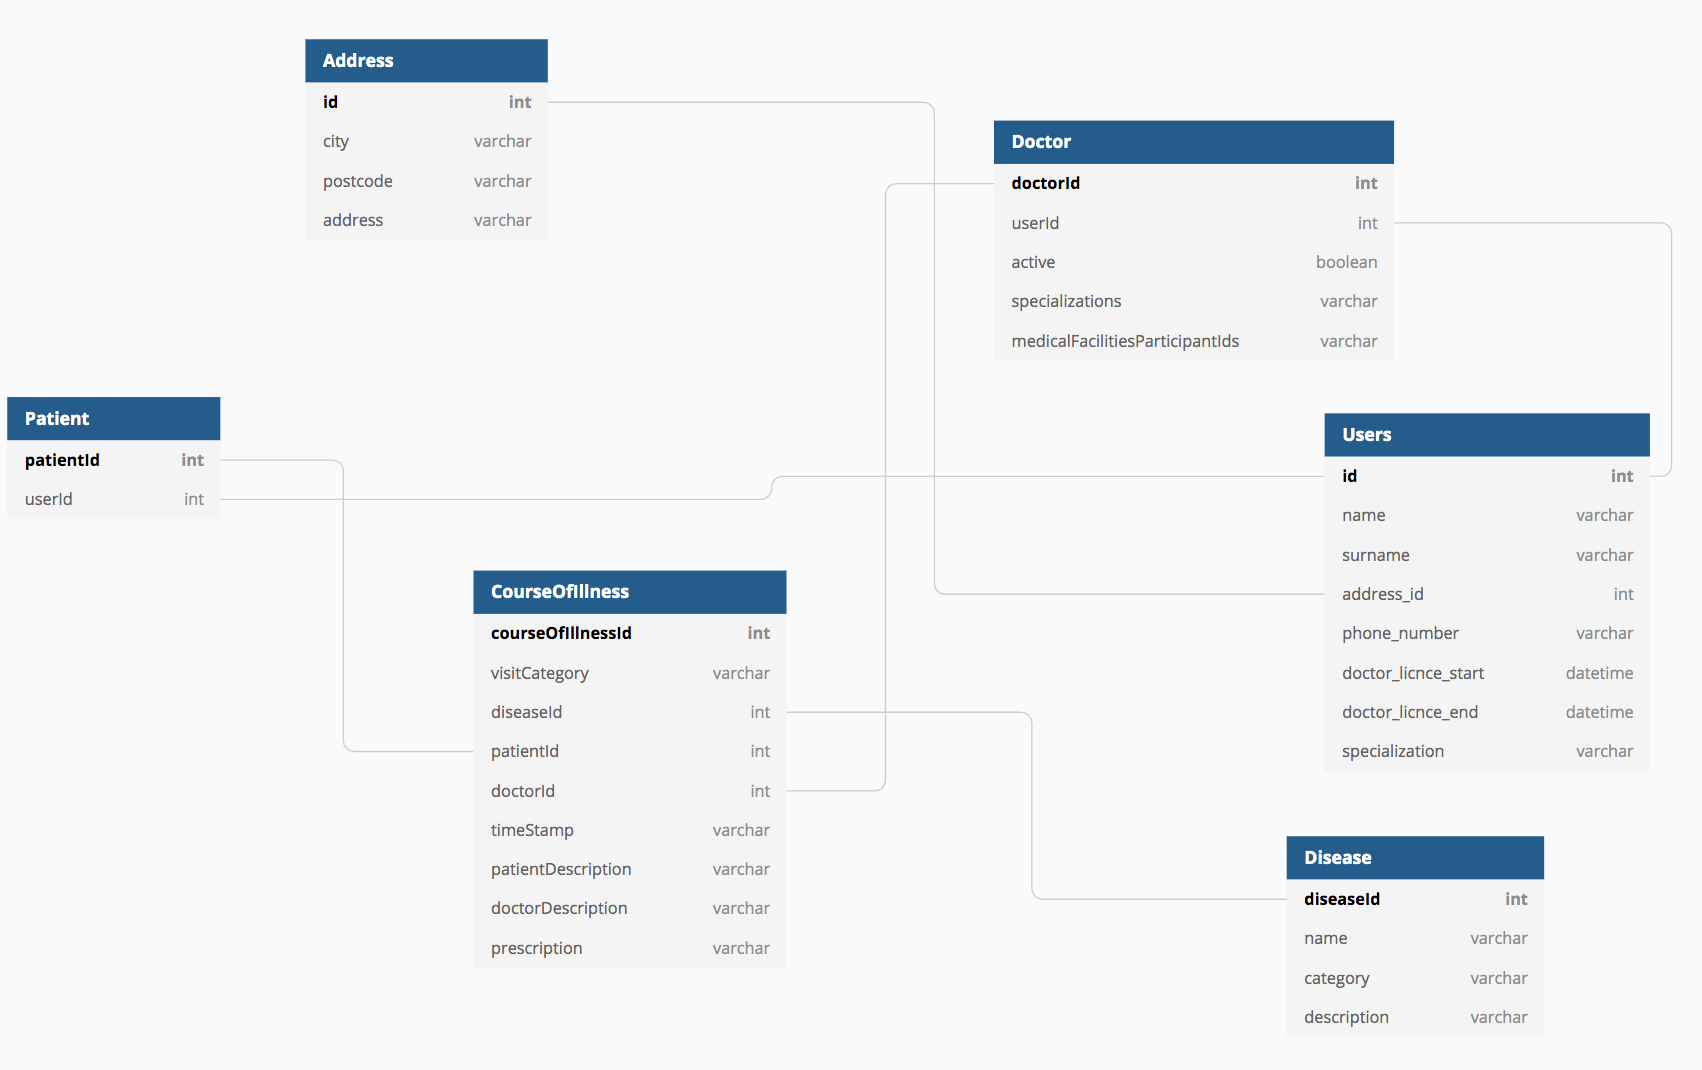
\includegraphics[width=15cm]{pictures/diagram}
\caption{Diagram ER bazy danych}
\end{figure}

\subsection{Aplikacja - backend}
\subsubsection{Endpointy}
Dzięki ogromnej popularności aplikacji internetowych opartych na języku \textit{Java} oraz \textit{framework Spring} możliwe było szybkie wygenerowanie dokumentacji \textit{Open API}. Pod \href{https://trunk-kartapacjentaservice.herokuapp.com/swagger-ui.html} {linkiem} dostępny jest spis wszystkich dostępnych w serwisie endpointów. Wejście w ten link będzie wymagało podania loginu i hasła (dostępnego tutaj: \ref{credentials}).

\subsubsection{Dlaczego REST?}
Zalety REST API:
\begin{itemize}
    \item Bezstanowość klienta - serwer nie ma potrzeby zapamiętywania wcześniejszego statnu, ponieważ zapytania HTTP zawierają wszystkie potrzebne informacje,
    \item Łatwość manipulowania obiektami z poziomu URL,
    \item Czytelność wykonywanych działań ze względu na Endpointy,
    \item Szybsze przetwarzanie informacji zwrotnej - uzycie JSON.
\end{itemize}

\subsubsection{Zabezpieczenie danych - API}
Większość \textit{endpointów} dostępnych w serwisie zapezpieczone jest przy użyciu metody \textit{Basic Auth}. Bez podania loginu i hasła niemożliwy jest dostęp do serwisu. Jedyne dostępne bez konieczności autoryzacji endpointy to te dotyczące logowania i rejestracji.

\subsubsection{Zabezpieczenie danych - baza danych}


\subsubsection{Ograniczenia}
\subsubsection{Możliwości dotyczące rozwoju - przyspieszenie}
\subsubsection{Rola serwera CRUD w aplikacji}

\subsection{Aplikacja - frontend}
\subsubsection{Działanie warstwy wizualnej}
\subsubsection{Prostota implementacji i wieloplatformowość}
\subsubsection{Rola warstwy wizualnej aplikcji}


\subsection{Testy obciążeniowe}
\subsubsection{Testowane zagadnienia}
\subsubsection{Wielowątkowość}
\subsubsection{Szybkość działania aplikacji}
\subsubsection{Rola testów w rozwoju aplikacji}

